% AY2021 制御工学 解答例
% 回答の流れ・言葉遣いは 03_制御工学/参考/「制御工学Ⅱ（完成版）」に寄せる。
% デザイン（囲み枠等）は真似しない。解答・数値は本年度過去問から自力で導いた。
\documentclass[11pt,a4paper]{article}
\usepackage{../../../00_common/preamble}

\usetikzlibrary{positioning,arrows.meta,calc}
\usepackage{pgfplots}
\pgfplotsset{compat=newest}

\title{制御工学 AY2021 解答例（専門応用科目I）}
\author{}
\date{}

\begin{document}
\maketitle

% ==================================================================
\section*{第1問〔I〕}

二次振動系（質量 $m$、粘性係数 $d$、バネ定数 $k$）。

\subsection*{(1) 運動方程式と伝達関数}
\begin{align*}
  &\qquad m\ddot{x}+d\dot{x}+kx=f(t)
   \quad\therefore\quad G(s)=\frac{1}{ms^2+ds+k}.
\end{align*}
\[
  \therefore\quad \ans{\;m\ddot{x}+d\dot{x}+kx=f(t),\qquad G(s)=\dfrac{1}{ms^2+ds+k}\;}
\]

\subsection*{(2) $d,k$ と定常値（$m=1,\omega_n=1,\zeta=0.5$）}
$\omega_n^2=\dfrac{k}{m}$、$2\zeta\omega_n=\dfrac{d}{m}$ より
\begin{align*}
  &\qquad k=m\omega_n^2=1,\qquad d=2\zeta\omega_n m=1.
\end{align*}
単位ステップ入力の定常値は、安定系では初期値によらず $x(\infty)=\lim_{s\to0}\dfrac{1}{s^2+s+1}=1$。
\[
  \therefore\quad \ans{\;d=1,\quad k=1,\quad x(\infty)=1\;}
\]

\subsection*{(3) 無減衰自由応答（$m=1,d=0,k=1$、$x(0)=1,\dot x(0)=0$）}
$f=0$ より $\ddot{x}+x=0$。$x=A\cos t+B\sin t$ に初期条件を入れて $A=1,B=0$。
\[
  \therefore\quad \ans{\;x(t)=\cos t\;}
\]
減衰がないので振幅 $1$ の持続振動となる。

\begin{center}
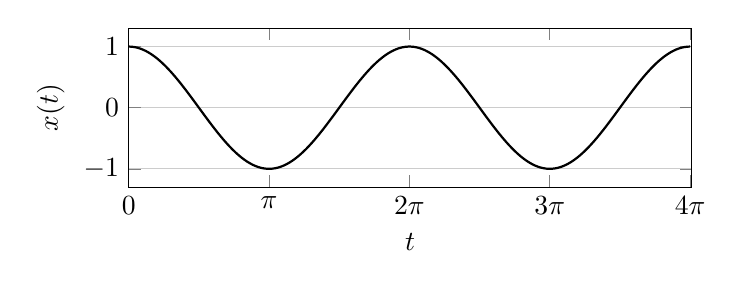
\begin{tikzpicture}
\begin{axis}[
  width=0.72\linewidth, height=3.6cm,
  xmin=0, xmax=12.6, ymin=-1.3, ymax=1.3,
  xlabel={$t$}, ylabel={$x(t)$},
  xtick={0,3.1416,6.2832,9.4248,12.566},
  xticklabels={$0$,$\pi$,$2\pi$,$3\pi$,$4\pi$},
  ytick={-1,0,1}, ymajorgrids=true, grid style={gray!40},
]
\addplot[thick,domain=0:12.566,samples=200]{cos(deg(x))};
\end{axis}
\end{tikzpicture}
\end{center}

\subsection*{(4) 指数入力応答（同パラメータ、$f(t)=\e^{-t}$、$x(0)=1,\dot x(0)=0$）}
$\ddot{x}+x=\e^{-t}$。特解 $x_p=C\e^{-t}$ より $2C\e^{-t}=\e^{-t}$、$C=\tfrac12$。
$x=\tfrac12\e^{-t}+A\cos t+B\sin t$ に初期条件を入れて
\begin{align*}
  &\qquad x(0)=\tfrac12+A=1,\qquad \dot{x}(0)=-\tfrac12+B=0
   \quad\therefore\quad A=B=\tfrac12.
\end{align*}
\[
  \therefore\quad \ans{\;x(t)=\tfrac12\e^{-t}+\tfrac12\cos t+\tfrac12\sin t\;}
\]
充分な時間が経つと $\e^{-t}\to0$ で定常項は $\tfrac12(\cos t+\sin t)=\dfrac{\sqrt2}{2}\sin\!\bigl(t+\tfrac{\pi}{4}\bigr)$。
よって振幅の最大値は
\[
  \therefore\quad \ans{\;|x(t)|_{\max}=\dfrac{\sqrt2}{2}\approx0.71\;}
\]
（(3) の振幅 $1$ より減少しており、振幅が抑えられている。）

\bigskip
\noindent 検算: (3)(4) とも導いた $x(t)$ が各微分方程式と初期条件を満たし、
(4) の定常項振幅 $\tfrac12\sqrt2=\tfrac{\sqrt2}{2}$ を SymPy で確認✓。

\newpage
% ==================================================================
\section*{第2問〔II〕}

$G_1,G_2,G_3$ を直列にし、$G_2$ の出力を $G_2$ 入力側へ（内側）、$G_2$ 入力点を入力側へ（外側）
それぞれ負帰還した系。

\subsection*{(1) 伝達関数}
$G_2$ 入力（$=$ sum2 出力）を $a$ とおく。内側帰還より $a(1+G_2)=G_1(\cdots)$、外側帰還より
$G_1$ 入力 $=U-a$ なので
\begin{align*}
  &\qquad a(1+G_2)=G_1(U-a)
   \quad\therefore\quad a(1+G_1+G_2)=G_1 U\\
  &\therefore\quad Y=G_3 G_2\,a=\frac{G_1G_2G_3}{1+G_1+G_2}\,U.
\end{align*}
\[
  \therefore\quad \ans{\;\dfrac{Y}{U}=\dfrac{G_1G_2G_3}{1+G_1+G_2}\;}
\]

\subsection*{(2) ゲインとゲイン線図（$G_1=\frac3s,\ G_2=\frac{1}{s+4},\ G_3=4$）}
\begin{align*}
  &\qquad \frac{Y}{U}=\frac{\frac3s\cdot\frac{1}{s+4}\cdot4}{1+\frac3s+\frac{1}{s+4}}
   =\frac{12/(s(s+4))}{(s^2+8s+12)/(s(s+4))}
   =\frac{12}{(s+2)(s+6)}.
\end{align*}
ゲインは
\[
  |T(j\omega)|_{\mathrm{dB}}=20\log_{10}\frac{12}{\sqrt{(12-\omega^2)^2+(8\omega)^2}},\qquad |T(0)|=1=0\,\mathrm{dB}.
\]
時定数形 $\dfrac{1}{(1+s/2)(1+s/6)}$ より折れ点は $\omega=2,\ 6$、傾きは $\omega<2$ で $0$、
$2<\omega<6$ で $-20$、$\omega>6$ で $-40\,[\mathrm{dB/dec}]$。

\begin{center}
\begin{tikzpicture}
\begin{axis}[
  width=0.86\linewidth, height=4.8cm,
  xmin=1e-1, xmax=1e3, ymin=-80, ymax=20, xmode=log,
  xlabel={$\omega\,[\mathrm{rad/s}]$}, ylabel={ゲイン [dB]},
  ytick={-80,-60,-40,-20,0,20},
  xmajorgrids=true, ymajorgrids=true, xminorgrids=true,
  grid style={line width=0.3pt, draw=gray!60},
  extra y ticks={0}, extra y tick style={grid=major, grid style={line width=1pt, draw=black}},
  legend pos=south west, clip=true, enlargelimits=false,
]
\addplot[thick] coordinates {(0.1,0) (2,0) (6,-9.5) (1000,-113.5)};
\addlegendentry{(2) $G_3=4$}
\addplot[thick,dashed] coordinates {(0.1,0) (6,0) (1000,-44.4)};
\addlegendentry{(4) $G_3=2s+4$}
\node[anchor=south] at (axis cs:2,0) {\scriptsize $\omega=2$};
\node[anchor=south west] at (axis cs:6,0) {\scriptsize $\omega=6$};
\end{axis}
\end{tikzpicture}
\end{center}

\subsection*{(3) ステップ応答（(2)）}
極は実数 $s=-2,-6$（過減衰）。$X(s)=\dfrac{T(s)}{s}$ を分解して
\begin{align*}
  &\qquad X(s)=\frac{12}{s(s+2)(s+6)}=\frac1s-\frac{1.5}{s+2}+\frac{0.5}{s+6}\\
  &\therefore\quad x(t)=1-1.5\,\e^{-2t}+0.5\,\e^{-6t}.
\end{align*}
オーバーシュートなく単調に立ち上がり、定常値 $1$ に収束する。支配極は $s=-2$（時定数 $0.5\,$s）。
\[
  \therefore\quad \ans{\;x(t)=1-1.5\,\e^{-2t}+0.5\,\e^{-6t}\;}
\]

\begin{center}
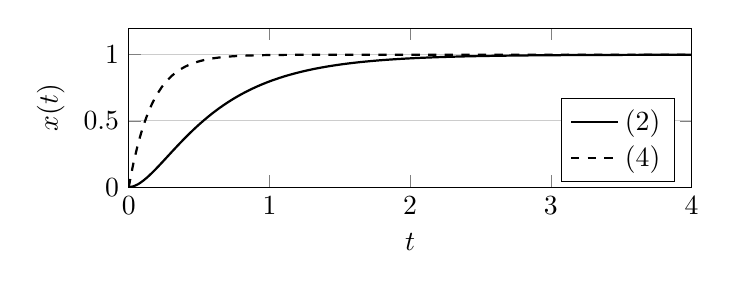
\begin{tikzpicture}
\begin{axis}[
  width=0.72\linewidth, height=3.6cm,
  xmin=0, xmax=4, ymin=0, ymax=1.2,
  xlabel={$t$}, ylabel={$x(t)$},
  ytick={0,0.5,1}, ymajorgrids=true, grid style={gray!40}, legend pos=south east,
]
\addplot[thick,domain=0:4,samples=120]{1-1.5*exp(-2*x)+0.5*exp(-6*x)};
\addlegendentry{(2)}
\addplot[thick,dashed,domain=0:4,samples=120]{1-exp(-6*x)};
\addlegendentry{(4)}
\end{axis}
\end{tikzpicture}
\end{center}

\subsection*{(4) $G_3=2s+4$ の場合の比較}
$G_3=2s+4=2(s+2)$ とすると分母 $1+G_1+G_2$ は不変で分子だけ変化し
\begin{align*}
  &\qquad T(s)=\frac{\frac3s\cdot\frac{1}{s+4}\cdot2(s+2)}{1+\frac3s+\frac{1}{s+4}}
   =\frac{6(s+2)}{(s+2)(s+6)}=\frac{6}{s+6}.
\end{align*}
零点 $s=-2$ が極 $s=-2$ を相殺して 1 次系になる。ステップ応答は
\[
  X(s)=\frac{6}{s(s+6)}=\frac1s-\frac{1}{s+6}
  \quad\therefore\quad \ans{\;x(t)=1-\e^{-6t}\;}
\]
\textbf{考察}：定常値はどちらも $1$ で不変だが、過渡特性は次のように変わる。
\begin{itemize}\setlength{\itemsep}{1pt}
  \item \textbf{時間応答}：(2) は遅い極 $s=-2$（$\tau=0.5\,$s）が支配したが、(4) ではこれが相殺され
        $s=-6$（$\tau\approx0.17\,$s）の 1 次系となり、整定が約 3 倍速い。
  \item \textbf{ゲイン線図}：(2) は折れ点 $\omega=2,6$ で最終傾き $-40\,$dB/dec だが、(4) は
        折れ点 $\omega=6$ のみ・傾き $-20\,$dB/dec で帯域が広がる（速い応答に対応）。
\end{itemize}

\bigskip
\noindent 検算: (2) $T=12/((s+2)(s+6))$・$|T(0)|=0\,$dB、(3) 単調増加で定常 $1$、
(4) 零点相殺で $T=6/(s+6)$・$x=1-\e^{-6t}$ を SymPy で確認✓。

\end{document}
